\section{OpenID for Verifiable Presentations (OID4VP)}
Questo standard definisce i meccanismi, basati sul OAuth 2.0 che permettono la presentazione di credenziali verificate ad un Verifier.

\subsection{Schema di Presentazione di una credenziale Same Device Flow}
Di seguito uno schema di interazione tra l'Holder e il Verifier, in cui interagiscono il Wallet e la parte che richiede una
certificazione del Verifier, entrambe sullo stesso Device.
\begin{center}
	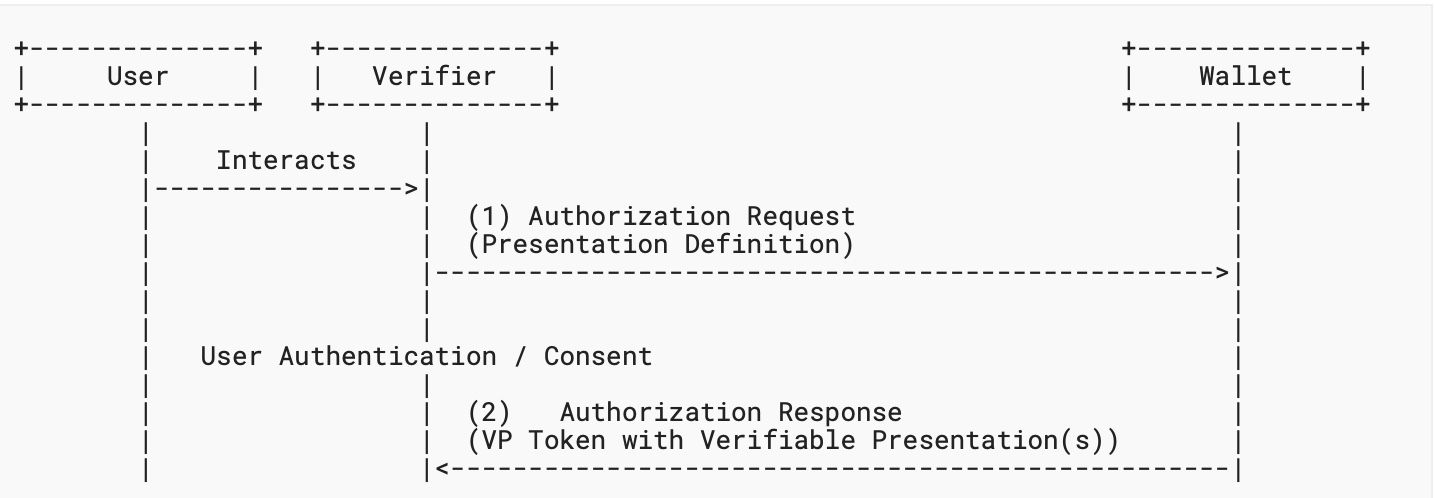
\includegraphics[scale = 0.3]{./res/images/PresentationSameDevice.jpg}
\end{center}

\subsection{Schema di presentazione di una credenziale Cross Device Flow}
Di seguito uno schema di interazione tra l'Holder con il proprio Wallet sul proprio device e il Verifer su un'altro device.\\

\begin{center}
	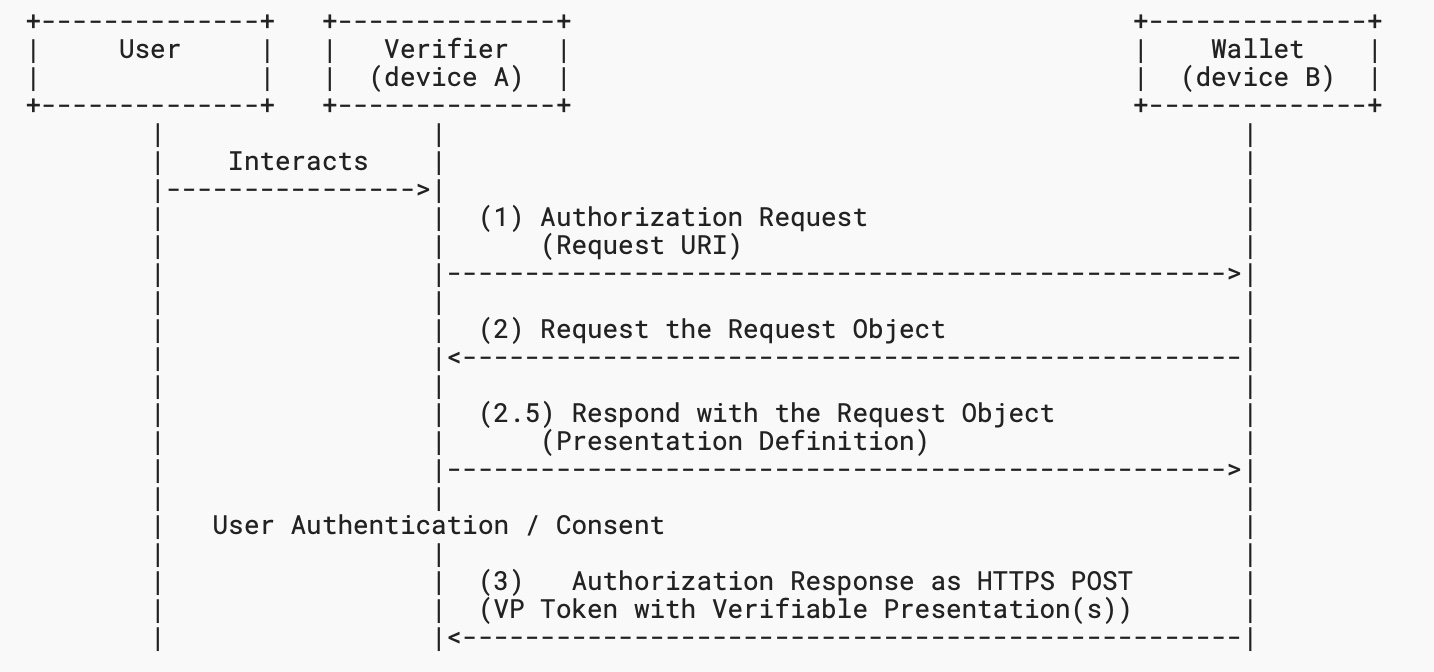
\includegraphics[scale = 0.3]{./res/images/PresentationCrossDevice.jpg}
\end{center}

\subsection{Authorization Request}
Un Verifier attraverso una definizione di presentazione definisce la presentazione che richiede.\\
Di seguito un esempio:
\begin{lstlisting}[language=json,firstnumber=1]
{
    "id": "vp token example",
    "input_descriptors": [
        {
            "id": "id card credential",
            "format": {
                "ldp_vc": {
                    "proof_type": [
                        "Ed25519Signature2018"
                    ]
                }
            },
            "constraints": {
                "fields": [
                    {
                        "path": [
                            "$.type"
                        ],
                        "filter": {
                            "type": "string",
                            "pattern": "IDCardCredential"
                        }
                    }
                ]
            }
        }
    ]
}
\end{lstlisting}
Durante la richiesta di Autorizzazione se è completata con successo il Verifier fornisce un VP Token al Holder.
\\
\subsection{Response}
Successivamente alla Authorization Request è fornito da parte del Verifier un VP Token.
Può essere ritornato al Authorization Response.
\\Di seguito un esempio di un VP Token Response:
\begin{lstlisting}[language=json,firstnumber=1]
{
    "@context": [
        "https://www.w3.org/2018/credentials/v1"
    ],
    "type": [
        "VerifiablePresentation"
    ],
    "verifiableCredential": [
        {
            "@context": [
                "https://www.w3.org/2018/credentials/v1",
                "https://www.w3.org/2018/credentials/examples/v1"
            ],
            "id": "https://example.com/credentials/1872",
            "type": [
                "VerifiableCredential",
                "IDCardCredential"
            ],
            "issuer": {
                "id": "did:example:issuer"
            },
            "issuanceDate": "2010-01-01T19:23:24Z",
            "credentialSubject": {
                "given_name": "Fredrik",
                "family_name": "Stromberg",
                "birthdate": "1949-01-22"
            },
            "proof": {
                "type": "Ed25519Signature2018",
                "created": "2021-03-19T15:30:15Z",
                "jws": "eyJhb...JQdBw",
                "proofPurpose": "assertionMethod",
                "verificationMethod": "did:example:issuer#keys-1"
            }
        }
    ],
    "id": "ebc6f1c2",
    "holder": "did:example:holder",
    "proof": {
        "type": "Ed25519Signature2018",
        "created": "2021-03-19T15:30:15Z",
        "challenge": "n-0S6_WzA2Mj",
        "domain": "https://client.example.org/cb",
        "jws": "eyJhbG...IAoDA",
        "proofPurpose": "authentication",
        "verificationMethod": "did:example:holder#key-1"
    }
}
\end{lstlisting}

\subsection{Response Mode direct\_post}
Esiste una modalità denominata Response Mode direct\_post che permette al Wallet di inviare Authorization Request 
direttamente ad un endpoint del Verifier via parametro HTTP POST. Questo metodo si usa quando Holder e Verifer sono su device diversi.

\subsection{Firma e Crittografia della Response}
L'Authorization Response contenente la VP Token può avere una Segnature cioè una firma e può essere crittograffata
a livello di applicazione nello schema TCP/IP.\\
Se si attuano queste pratiche attraverso la crittografia si può prevenire la leak di dati e con la firma si può avere la certezza che 
i dati al suo interno sinao originali.

\subsection{VP Token Validation}
Un Verifier deve validare un VP Token.Deve garantire integrità, autenticità e binding dell'Holder con qualsiasi presentazione che sta cercando di fornire.Verificare che la presentazione rispetti i formatti richiesti.

\subsection{Wallet Metadata}
Il Verifier può accedere ad informazioni come il formato delle credenziali, tipo di proof, ed in generale gli algoritmi supportati.
